\documentclass[11pt]{article}
%%% PAGE DIMENSIONS
\usepackage{geometry} % to change the page dimensions
\geometry{a4paper} % or letterpaper (US) or a5paper or....
\geometry{margin=1.25in, left=0.75in, right=0.75in, headheight = 14pt} % for example, change the margins to 2 inches all round
% \geometry{landscape} % set up the page for landscape
%   read geometry.pdf for detailed page layout information
\usepackage{graphicx} % support the \includegraphics command and options
\usepackage{longtable}
\usepackage{float}
\usepackage{wrapfig}
\usepackage{multicol}
\usepackage{multirow}
\usepackage[normalem]{ulem}
\usepackage[table,xcdraw]{xcolor}

\usepackage[parfill]{parskip} % Activate to begin paragraphs with an empty line rather than an indent

%%% PACKAGES
\usepackage{booktabs} % for much better looking tables
\usepackage{array} % for better arrays (eg matrices) in maths
\usepackage{paralist} % very flexible & customisable lists (eg. enumerate/itemize, etc.)
\usepackage{verbatim} % adds environment for commenting out blocks of text & for better verbatim
\usepackage{subfig} % make it possible to include more than one captioned figure/table in a single float
% These packages are all incorporated in the memoir class to one degree or another...

\usepackage{listings}

\DeclareUnicodeCharacter{200A}{-} 


%%% TITLE AND AUTHOR

\title{ 
    ELE00017M | Top Three Uses of Neural Networks in Voice Research
}

\author{Nathan Billis}
%\date{} % Activate to display a given date or no date (if empty),
         % otherwise the current date is printed 
\makeatletter

%%% HEADERS & FOOTERS
\usepackage{fancyhdr} % This should be set AFTER setting up the page geometry
\pagestyle{fancy} % options: empty , plain , fancy
\renewcommand{\headrulewidth}{1pt} % customise the layout...
\lhead{\@title}\chead{}\rhead{\@author}
\lfoot{}\cfoot{\thepage}\rfoot{}


%%% SECTION TITLE APPEARANCE
\usepackage{sectsty}
\allsectionsfont{\sffamily\mdseries\upshape} % (See the fntguide.pdf for font help)
% (This matches ConTeXt defaults)

%%% ToC (table of contents) APPEARANCE
\usepackage[nottoc,notlof,notlot]{tocbibind} % Put the bibliography in the ToC
\usepackage[titles,subfigure]{tocloft} % Alter the style of the Table of Contents
\renewcommand{\cftsecfont}{\rmfamily\mdseries\upshape}
\renewcommand{\cftsecpagefont}{\rmfamily\mdseries\upshape} % No bold!

% biblatex for citations
\usepackage{csquotes}
\usepackage[backend=biber,citestyle=ieee]{biblatex}
\addbibresource{references.bib}
\usepackage{url}

\usepackage[colorlinks=false, allbordercolors={0 0 0},pdfborderstyle={/S/U/W 1}]{hyperref}

\graphicspath{{images/}}

\begin{document}
\begin{titlepage}
    \centering
    {\scshape\LARGE department of electronics \par}
    \vspace{0.5cm}
    {\scshape\Large biologically inspired computing \par}
    \vspace{0.5cm}
    {\scshape\Large ele00017m \par}
    \vspace{2.5cm}
    {\scshape\Large top three uses of neural networks in voice research \par}
    % maybe an image here
    \vfill
    {\Large\itshape \@author \par}
    \vspace{2cm}
    
    \tableofcontents

\end{titlepage}

\pagenumbering{arabic} % Start arabic numbering
	
\newpage

    \section{Introduction}
    
    Voice research is currently a very important research area, especially with the rise of smart speakers such as the Amazon Echo \cite{IntroducingRoom}, Google Nest \cite{GoogleStore} and Apple Homepod \cite{HomePodUK}. The importance of accurate voice recognition is not only important from an accessibility standpoint but also for people using these devices. 
    
    Speech has been an important way of communicating with each other and although speech recognition has moved alot very quickly it's still not perfect. When working with speech there are a variety of different issues. Some of the most common issues include \cite{Gevaert2010NeuralRecognition}: 
    \begin{itemize}
        \item Speaker Variation: where the same words are pronounced differently by diff rent people because of variations with gender, age, speed of speech and many other tiny changes.
        \item Background Noise: where the event is noisy it can add to the signal and even the speaker can add unwanted noise to the signal.
        \item Continuous Speech: when we speech there are occasions where there are no breaks between words making it difficult to disguise the start and ends of words.
        \item Other External Factors: in addition to the issues above there can be a variety of other factors such as the position of the microphone all having a knock on effect on the quality of the recording.
    \end{itemize}
    
    This report will look at why Automatic Speech Recognition, Large Vocabulary Speech Recognition, and Noise Robust Speech Recognition are the top three applications of neural networks within voice research.
    
    \section{Neural Networks Overview}
    Neural networks (NN) are the most common form of biologically inspired computing in the real world. There are many types of Neural Networks each having their own advantages and disadvantages. Many are treated as a black box style model with inputs on one side and outputs on the other, and they all generally require alot of training to present good results.
    
    \begin{figure}[h]
        \centering
        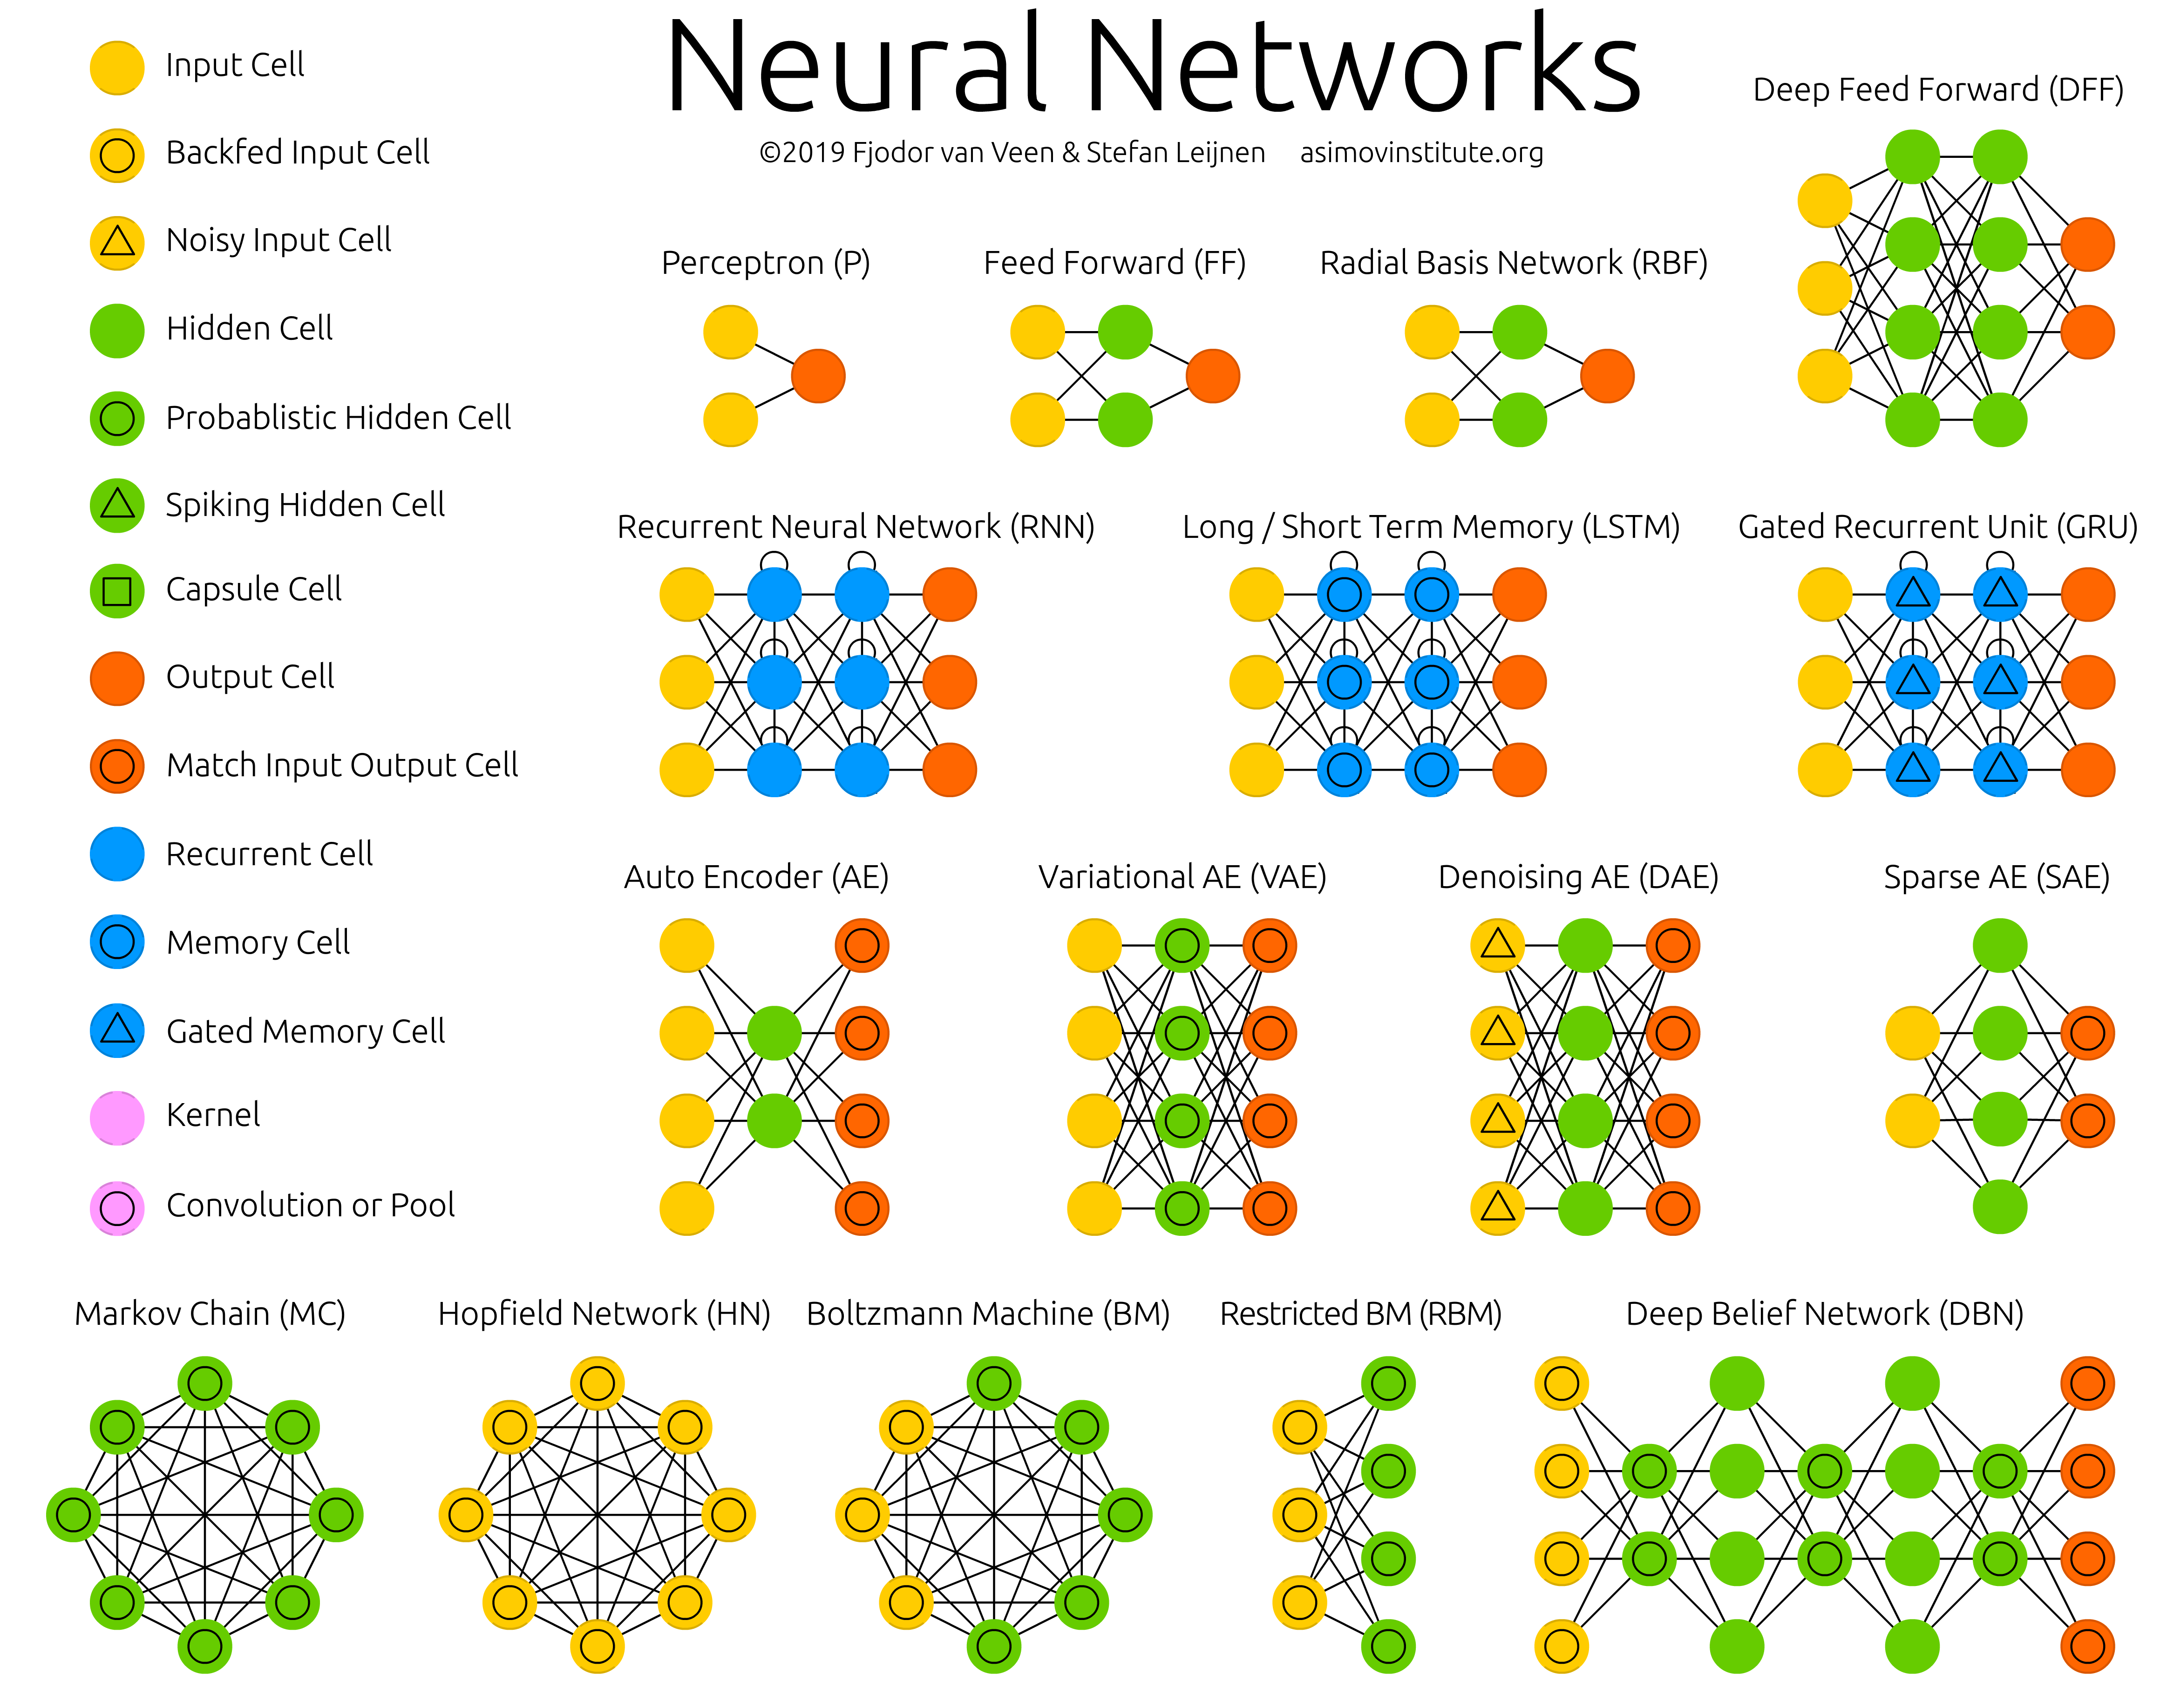
\includegraphics[scale=0.1]{NeuralNetwork.png}
        \caption{Main Types of Neural Networks \cite{Leijnen2020TheZoo}}
        \label{fig:neuralNetworks}
    \end{figure}
    
    Figure \ref{fig:neuralNetworks} displays some of the popular neural network types. Each network has differing strengths and because of this they're adapted for their differing uses. The two main networks that are used in voice research are Feed Forward Network (FF) and Recurrent Neural Network (RNN), other types of networks are used however these two are the main one's we'll be focusing on. Neural Networks are made up of connected processes called neurons \cite{Schmidhuber2015DeepOverview}, each being activated in different ways with input nodes being activated by the environment. The complexity of the problem changes how many computational stages there needs to be in the network.
    
    \subsection{Feed Forward}
    When we combing many neurons we create a network, and depending on the configuration changes the network type. The most basic is feed forward networks (FF). FF are arranged in layers \cite{NeuralArchitecture}, with each layer leading to the next layer and then onto the output. Unlike other forms of neural networks there are no connections between layers. The connection between each layer has differing weights and bias changing the result of the output.
    
    FF tend to "learn" from training and don't adapt after the initial training phase, the weights and bias which are created during the training phase remain for the duration of the networks existence. These networks are used for supervised machine learning where we know what the outputs should be. 
    
    \subsection{Recurrent Neural Networks}
    Recurrent neural networks (RNN) are similar to feed forward networks however unlike FF they learn from the past \cite{RecurrentScience} and their decisions are influenced by that in addition to training. RNN are useful when the data needs to look at around the key item of interest. This is because RNN not only have access to their own node but also those around it. This makes it useful for looking at things like the next word in a sentence because it's important to have the words that come before in order to use it in context.
    
        \begin{figure}[h]
        \centering
        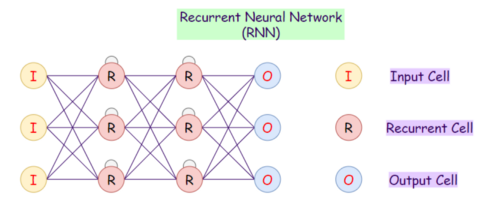
\includegraphics[scale=0.75]{RNN.png}
        \caption{Recurrent Neural Network \cite{MainAI}}
        \label{fig:RRN}
    \end{figure}
    
    Because the network operates in layers the order is important. When training these networks it is possible information may get lost over time, due to a vanishing or exploding gradient which is where the weights and bias are against the correct output causing data loss.
    
    \pagebreak
    
    \section{Automatic Speech Recognition (ASR)}
    
    One of the top uses of NN in voice research is within ASR. Before using neural networks in ASR, it relied heavily on statistical models such as hidden markov models. Neural networks are already used in devices such as the Amazon Echo \cite{SwarupImprovingEmbeddings} and help to reduce the word error rate.
    
    \subsection{Phonemes and Voice Acoustics}
    Before looking at how ASR works it helps to have an understanding on Voice Acoustics. The best place to start is by first looking at phonemes, phonemes are a basic linguistic "unit" and every word is made up a series of phonemes, phonemes are not the same as syllables and if you change a phoneme you change the word. Phonemes are described from where they are produced in the mouth. The International Phonetic Alphabet is a system of phonetic notations that quantifies the speech that forms oral language. 
    
    \begin{figure}[h]
        \centering
        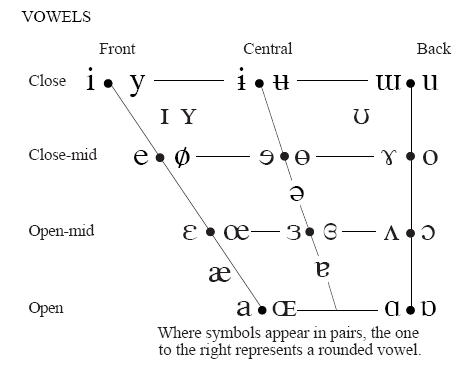
\includegraphics[scale=0.5]{vowels.png}
        \caption{IPA: vowels \cite{InternationalPhoneticAssociationIPA:Association}}
        \label{fig:vowles}
    \end{figure}
    
    Each phoneme has a unique spectral signature based on the format making it easier to identify. Where two vowels are next to each other that creates a diphthong which again has a slightly different spectral signature. The data from speech can be represented in several different ways depending on it's intended use, this can be a Waveform, a Spectogram or Mel Frequency Cepstrum Coefficients. 
    
    The approximate formula to calculate mels for a frequency in Hz \cite{Gevaert2010NeuralRecognition}:
    
    \begin{equation}
    mel(f)=2595.^{10} log(1+ \frac{f}{700})
    \end{equation}

   When looking at feature extraction from speech Mel Frequency Cepstrum Coefficients analysis (MFCC) is a popular choice because it generally allows the same result irrespective of any time dependant problems. It has a much higher recognition success rate with used in combination with other methods of feature extraction such as using linear prediction co-efficients or Power Spectral Density points \cite{Moonasar2001ASystems}. Before the signal enters the neural network some pre-processing is done to the signal to clean it up and get it into a format that will be easier understood by the network.

    \subsection{ASR and neutral networks}
    After gaining a basic understanding of the functions of phonemes in the speech chain it's now possible to look at Automatic Speech Recognition (ASR) and why phonemes are so important in it's usage and why neural networks are used.
    
    Feedforward Networks (FF) using Back Propagation algorithm for training is a popular network for ASR \cite{K.R2016AutomaticSurvey}, RNN are also quite popular. FF neural networks need a constant input to ensure the output will be as expected because of this the all of the data from the full spectrograms is not used as an input and instead the MFCC, as discussed earlier, is used. Because the MFCC is used the dataset is alot smaller meaning that the calculations and training are alot quicker. 
    
    Depending on the number of words we want to recognise, the size of the network and number of output nodes will change. To estimate the number of neurons needed in the network Oja rule of thumb \cite{Oja1982SimplifiedAnalyzer} is used:
    
    \begin{equation}
    H = \frac{T}{5(N+M)}
    \end{equation}
    
    Where H is the number of hidden layer neurons, N is the input later size, M the output layer size, and T is the size of the training set. After we've created the network it can be trained using supervised training and then used to classify words. From this equation we see that with more words in the dictionary the bigger the network needs to become.
    
    The shift from using statistical models or hybrid methods has allowed ASR to become more accurate and have a higher confidence level. Neural networks are very powerful at classifying speech and work well when paired with good pre-processing such as using Mel Frequency Cepstrum Coefficients over spectrograms.
    

    \section{Large Vocabulary Speech Recognition}
    Another use of neural networks in voice research is for large vocabulary speech recognition, when looking at ASR we discussed how having a large dataset meant that the neural network would be reasonably large, because of this different approaches have to be taken when looking at large vocabulary speech recognition.
    
    RNNs
    
    
    \section{Noise Robust Speech Recognition}
    
    250
    
    \section{Conclusion}
    250
    \begin{itemize}
        \item why are these the top uses
        \item what did we find in the paper
        \item further discussion points
    \end{itemize}
    
        


\pagebreak

\printbibliography


\end{document}